\section{Homogeneous vs non-homogeneous}

\subsection*{Resources}
\begin{itemize}
    \item Page 1 of the PDF \url{http://www.math.psu.edu/tseng/class/Math251/Notes-LinearSystems.pdf}
\end{itemize}

\subsection*{Challenge}
Separately add the points of the following \emph{homogeneous} and \emph{non-homogeneous} ODE systems:

1 point:
$\displaystyle
\left(
    \begin{array}{c}
        x_1' \\
        x_2' \\
        x_3'
    \end{array}
\right)
=
\left(
    \begin{array}{ccc}
        1 & 2 & 3 \\
        4 & 5 & 6 \\
        7 & 8 & 9
    \end{array}
\right)
\left(
    \begin{array}{c}
        x_1 \\
        x_2 \\
        x_3
    \end{array}
\right)
+
\left(
    \begin{array}{c}
        0 \\
        0 \\
        0
    \end{array}
\right)
$

2 points:
$\displaystyle
\left(
    \begin{array}{c}
        x_1' \\
        x_2' \\
        x_3'
    \end{array}
\right)
=
\left(
    \begin{array}{ccc}
        1 & 2 & 3 \\
        4 & 5 & 6 \\
        7 & 8 & 9
    \end{array}
\right)
\left(
    \begin{array}{c}
        x_1 \\
        x_2 \\
        x_3
    \end{array}
\right)
+
\left(
    \begin{array}{c}
        Cos(t) \\
        0 \\
        0
    \end{array}
\right)$

4 points:
$\displaystyle
\left(
    \begin{array}{c}
        x_1' \\
        x_2' \\
        x_3'
    \end{array}
\right)
=
\left(
    \begin{array}{ccc}
        1 & 2 & 3 \\
        4 & 5 & 6 \\
        7 & 8 & 9
    \end{array}
\right)
\left(
    \begin{array}{c}
        x_1 \\
        x_2 \\
        x_3
    \end{array}
\right)
+
\left(
    \begin{array}{c}
        Cos(t) \\
        Sin(t) \\
        0
    \end{array}
\right)$

8 points:
$\displaystyle
\left(
    \begin{array}{c}
        x_1' \\
        x_2' \\
        x_3'
    \end{array}
\right)
=
\left(
    \begin{array}{ccc}
        1 & 2 & 3 \\
        4 & 5 & 6 \\
        7 & 8 & 9
    \end{array}
\right)
\left(
    \begin{array}{c}
        x_1 \\
        x_2 \\
        x_3
    \end{array}
\right)
+
\left(
    \begin{array}{c}
        Cos(t) \\
        Sin(t) \\
        Tan(t)
    \end{array}
\right)$

\subsection*{Solution}
Homogeneous: \hash{hhh}{106c67} \\
Non-homogeneous: \hash{iii}{d51f57}




%%%%%%%%%%%%%%%%%%%%%%%%%%%%%%%%
\newpage
%%%%%%%%%%%%%%%%%%%%%%%%%%%%%%%%
\section{Basis for creating a system of equations from a single ODE}
\label{sec:systembasis}

\subsection*{Resources}
\begin{itemize}
    \item Pages 1-4 of the PDF \url{http://www.math.psu.edu/tseng/class/Math251/Notes-LinearSystems.pdf} 
\end{itemize}

\subsection*{Comment}
\emph{Note that the notation $y^{(2)}$ means ``the 2nd differential of y'' while the notation $y^2$ (without the brackets around the $2$) means ``y-squared''.}

Considering the general form of an nth-order linear equation,
\begin{equation}
    a_n y^{(n)} + a_{n-1} y^{(n-1)} + \cdots + a_1 y^{(1)} + a_0 y = g(t)
\end{equation}
we substitute $x_1=y$, $x_2=y'$, \ldots, $x_n=y^{(n-1)}$ and $x_n'=y^{(n)}$.

When replacing a $y$-term by an $x$ term, the $n$ in $x_n$ corresponds to one more than the number of times $y$ is differentiated. So $x_{n+1}$ corresponds to $y$ being differentiated $n$ times and $x_n$ corresponds to $y$ being differentiated $n-1$ times. So $x_2$ corresponds to $y^{(1)}$ (differentiated 1 time) and $x_1$ corresponds to $y$ (differentiated 0 times).

Note that $x_n'$ is one more differential than $x_n$, so $x_n'$ corresponds to $(y^{(n-1)})' = y^{(n)}$.
So the $n$ in $x_n'$ corresponds to the number of times $y$ is differentiated (ie, $y^{(n)}$).

The examples on page 3 are clearer after reading page 4, so I encourage you to read page 4 before considering the examples.

Considering example (II) on page 3, you are given the equation
\begin{equation}
    y''' - 2y'' + 3y' - 4y = 0
\end{equation}

To add a more detailed explanation to that found in the PDF: First re-write the ODE in terms of $x$ and $x'$. Note that there is no ``$x_0'$'' so we just write it as $x_1$ in both equations.
\begin{align}
    x_4 - 2 x_3 + 3 x_2 - 4 x_1 &= 0 \label{eq:xs} \\
    x_3' - 2 x_2' + 3 x_1' - 4 x_1 &= 0 \label{eq:xprimes}
\end{align}

Our aim is to write the system of equations in the form $\bm{x'} = \bm{A}\bm{x}$. Note that there is no ``$x_4'$'' in our equations, so the largest value of $n$ in $x_n'$ will be 3 (ie, $x_3'$).
\begin{equation}
    \left(
        \begin{array}{c}
            x_1' \\
            x_2' \\
            x_3'
        \end{array}
    \right)
    =
    \left(
        \begin{array}{ccc}
            ? & ? & ? \\
            ? & ? & ? \\
            ? & ? & ?
        \end{array}
    \right)
    \left(
        \begin{array}{c}
            x_1 \\
            x_2 \\
            x_3
        \end{array}
    \right)
\end{equation}
where the question marks are values that we have to find.

By direct comparison of equations \ref{eq:xs} and \ref{eq:xprimes} we know that $x_1' = x_2$ which can be written as $x_1' = 0 x_1 + 1 x_2 + 0 x_3$ yielding the first line in the matrix $\bm{A}$:
\begin{equation}
    \left(
        \begin{array}{c}
            x_1' \\
            x_2' \\
            x_3'
        \end{array}
    \right)
    =
    \left(
        \begin{array}{ccc}
            0 & 1 & 0 \\
            ? & ? & ? \\
            ? & ? & ?
        \end{array}
    \right)
    \left(
        \begin{array}{c}
            x_1 \\
            x_2 \\
            x_3
        \end{array}
    \right)
\end{equation}

We can then proceed to do $x_2$ in a similar fashion:
\begin{equation}
    \left(
        \begin{array}{c}
            x_1' \\
            x_2' \\
            x_3'
        \end{array}
    \right)
    =
    \left(
        \begin{array}{ccc}
            0 & 1 & 0 \\
            0 & 0 & 1 \\
            ? & ? & ?
        \end{array}
    \right)
    \left(
        \begin{array}{c}
            x_1 \\
            x_2 \\
            x_3
        \end{array}
    \right)
\end{equation}

In order to express $x_3'$ in the above matrix form, we need it in terms of $x_1$, $x_2$ and $x_3$ rather than $x_4$, so instead of direct comparison, we swap $x_4$ for $x_3'$ in equation \ref{eq:xs} to read
\begin{equation}
    x_3' - 2 x_3 + 3 x_2 - 4 x_1 = 0
\end{equation}
and then isolate $x_3'$ to read $x_3' = 4 x_1 - 3 x_2 + 2 x_3$ yielding the final form of our systems of equations
\begin{equation}
    \left(
        \begin{array}{c}
            x_1' \\
            x_2' \\
            x_3'
        \end{array}
    \right)
    =
    \left(
        \begin{array}{ccc}
            0 & 1 & 0 \\
            0 & 0 & 1 \\
            4 & -3 & 2
        \end{array}
    \right)
    \left(
        \begin{array}{c}
            x_1 \\
            x_2 \\
            x_3
        \end{array}
    \right)
\end{equation}

Note that this is only considering a homogeneous equation. If it is non-homogeneous, you will have an extra term in the final step and will need a matrix of the form  $\bm{x'} = \bm{A}\bm{x} + \bm{g}$ as shown in the answer to exercise 4(b) on page 5 of the PDF.

So why do we want to do this? Well, notice that in this example we started with a complicated 3rd-order ODE and reduced it into 3 1st-order ODE's. Similarly, if we started with a 2nd-order ODE, we could reduce the equation to 2 1st-order ODE's. In general, for an nth-order ODE we can reduce it to $n$ 1st-order ODE's. If we can then learn how to solve simultanious sets of 1st-order ODE's, we have a powerful method of increasing our understanding (and even solving) difficult higher-order ODE's. 

Similarly, if you are given a system of 2 1st-order ODE's, you can know that it can form a single 2nd-order ODE. 

\subsection*{Challenge}
Write the following ODE's in matrix form:

1) $2 y'' + 4 y' - 6 y = 0$

2) $y'' + y = Cos(t)$

Complete exercises 1 and 2 on page 5 of the PDF.

\subsection*{Solutions}
To check your answers, sum the values of all the terms in your matrix $\bm{A}$.

1) 2

2) 0 (remember there is also a $+\bm{g}$ column-vector added to $\bm{A}\bm{x}$ too)

The answers to the PDF exercises are shown on page 5 of the PDF. Perhaps obviously, since you will not have the answers in a real-life/exam environment, please don't review each answer until completion. If you get stuck, be sure to review your notes (especially the worked-examples in the PDF) rather than the answers, to facilitate deep learning. 




%%%%%%%%%%%%%%%%%%%%%%%%%%%%%%%%
\newpage
%%%%%%%%%%%%%%%%%%%%%%%%%%%%%%%%
%\input{matricies}
\section{Matricies}

\subsection*{Resources}
\begin{itemize}
    \item PDF: Pages 6-17 of the PDF \url{http://www.math.psu.edu/tseng/class/Math251/Notes-LinearSystems.pdf}
\end{itemize}

\subsection*{Comment}
It is worth spending some time getting comfortable with manipulating matricies, since this is an indispensible basis for the work that is about to follow. The PDF gives a quick introduction to matricies. For a more thorough introduction, the Khan Academy playlist on linear algebra [1] is excellent, although beyond the scope of this course.

One note to deal with any confusion arising with regard to eigenvectors with matricies with zeros. For $(A-rI)$ equal to something like
\begin{equation}
\left(
    \begin{array}{cc}
        0 & 0 \\
        1 & 2
    \end{array}
\right)
\end{equation}
the top row can be ignored since any $x_1$ and $x_2$ will satisfy the top row.

Similarly, for a case such as
\begin{equation}
\left(
    \begin{array}{cc}
        2 & 0 \\
        2 & 0
    \end{array}
\right)
\end{equation}
you will have
\begin{align}
    2 x_1 + 0 x_2 &= 0 \\
    2 x_1 &= 0 \\
    x_1 &= 0
\end{align}
which is satisfied by
\begin{equation}
\left(
    \begin{array}{c}
        0 \\
        1
    \end{array}
\right)
\end{equation}
(where the $1$ could in principle be any number, but is the minimum integer that satisfies the condition.)

Finally, note that $(A-rI) = ((a, b), (c, d))$ will give you two equivalent formulas $a x_1 + b x_2 = 0$ and $c x_1 + b x_2 = 0$, even if they may appear different on first glance. If you want, you can prove to yourself that they are the same by multiplying the bottom row by $a/c$.

\vspace{0.2cm}
\noindent [1] \url{https://www.khanacademy.org/math/linear-algebra/alternate-bases}

\subsection*{Challenges}
Complete exersizes 1, 2, 3, 4 (I and II only) and 5 on page 18 of the PDF.

\subsection*{Solutions}
The answers to the PDF exercises are shown on page 18 of the PDF. Perhaps obviously, since you will not have the answers in a real-life/exam environment, please don't review each answer until completion. If you get stuck, be sure to review your notes (especially the worked-examples in the PDF) rather than the answers, to facilitate deep learning. 

The solution to question 1 above can be found on the next page.




%%%%%%%%%%%%%%%%%%%%%%%%%%%%%%%%
\newpage
%%%%%%%%%%%%%%%%%%%%%%%%%%%%%%%%
\section{Eigenvector equivalence}

\subsection*{Comment}
Considering the matrix
\begin{equation}
    A = \left(
        \begin{array}{cc}
            1 & 2 \\
            -3 & -4
        \end{array}
    \right)
\end{equation}
The eigvenvalues are -2 and -1. Considering the eigenvalue -2, 
\begin{equation}
    A - Ir = \left(
        \begin{array}{cc}
            3 & 2 \\
            -3 & -2
        \end{array}
    \right)
\end{equation}
To determine the eigenvector we can either take the top or bottom row in the calculation $(A - Ir)x = 0$.
The top and bottom row appear with different numbers but it is easy to see that they yield multiples of the same eigenvector and are therefore equivalent.

Complex eigenvectors are no different, but it can sometimes be hard to see that they are indeed equivalent.

\subsection*{Challenge}
Show that the equation $(A - Ir)\bm{x} = {0}$, where
\begin{equation}
     A-Ir = \left(
        \begin{array}{cc}
            -3 -3i & 6 \\
            -3 & 3-3i
        \end{array}
    \right)
\end{equation}
yields the same eigenvector, irrespective of whether you calculate the eigenvector using the top or bottom row of $(A-Ir)$. You may find that one of the representations of the eigenvectors looks like $(i-1,1)$.

\subsection*{Solutions}
You should be able to generate two eigenvectors by using the top and bottom rows of the $A-Ir$ matrix, and show that they are infact the same eigenvector by multiplying by an equivalent (imaginary) number. Please discuss with your partner or the teacher in class if you have trouble.



%%%%%%%%%%%%%%%%%%%%%%%%%%%%%%%%
\newpage
%%%%%%%%%%%%%%%%%%%%%%%%%%%%%%%%
\section{Solving systems of ODE's}
\label{sec:systemsolving}

\subsection*{Resources}
\begin{itemize}
    \item Pages 6-31 of the PDF \url{http://www.math.psu.edu/tseng/class/Math251/Notes-LinearSystems.pdf} 
\end{itemize}

\subsection*{Challenge}
Complete at least exercises 1-10 on page 32-33 of the PDF.

\subsection*{Solutions}
It might not be clear to you why solutions involve vectors and what this means physically, but for now, please just get used to solving equations in this fashion.

The answers are shown on page 33-34 of the PDF. Perhaps obviously, since you will not have the answers in a real-life/exam environment, please don't review each answer until completion. If you get stuck, be sure to review your notes (especially the worked-examples in the PDF) rather than the answers, to facilitate deep learning. 

%NT: Add something about intersection of graphs? https://en.wikipedia.org/wiki/System_of_linear_equations
% Good resources: http://www.math.psu.edu/tseng/class/Math251/




%%%%%%%%%%%%%%%%%%%%%%%%%%%%%%%%
\newpage
%%%%%%%%%%%%%%%%%%%%%%%%%%%%%%%%
\section{Graphs of system solutions}

\subsection*{Resources}
In the previous challenge you determined $x_1$ and $x_2$ with solutions such as
\begin{equation}
    \bm{x} = \matrixcrr{x_1}{x_2} = c_1 \matrixcrr{-1}{6} e^{-6t} + c_2 \matrixcrr{1}{1} e^t
\end{equation}

or written another way:
\begin{align}
    x_1 &= -c_1 e^{-6t} + c_2 e^t \label{eqn:sysgraphx1} \\
    x_2 &= 6 c_1 e^{-6t} + c_2 e^t \label{eqn:sysgraphx2} 
\end{align}

This particular system arose from a 2nd-order differential equation:
\begin{equation}
    y'' + 5y' - 6y = 0 \label{eqn:sys2ndoode}
\end{equation}

we have learned in challenge \ref{sec:systembasis} that this 2nd-order equation can be written in terms of $x$:

\begin{equation}
    x_3 + 5x_2 - 6 x_1 = 0
\end{equation}

Thus we remember that $x_1 = y$ and $x_2 = y'$, allowing equations \ref{eqn:sysgraphx1} and \ref{eqn:sysgraphx2} to be written as
\begin{align}
    y &= -c_1 e^{-6t} + c_2 e^t \label{eqn:syspos} \\
    y' &= 6 c_1 e^{-6t} + c_2 e^t \label{eqn:sysvel} 
\end{align}

Perhaps, for example, the original 2nd-order ODE (equation \ref{eqn:sys2ndoode}) represented the position of an atom on an axis with respect to time. Then equation \ref{eqn:syspos} represents position at time $t$ while equation \ref{eqn:sysvel} represents the velocity (or more commonly, when multiplied by the mass, represents the momentum).

Thus the graph represents the variation of momentum (velocity) with position, called the ``phase-space'' of the system. A specific trajectory can be followed given boundary conditions that determine the starting condition. For example, if the particle at time $t=0$ is known to have position $y=1$ and velocity $y'=2$ we can impose the boundary condition
\begin{equation}
    \bm{x}(0) = \matrixcrr{1}{2}
\end{equation}
to determine the coefficients $c_1$ and $c_2$ and obtain a unique trajectory.

We can then plot the phase-space for various boundary conditions. In the graph below, we show examples where $c_1 = c_2 = \{0, 0.5, 1, 1.5, 2\}$:

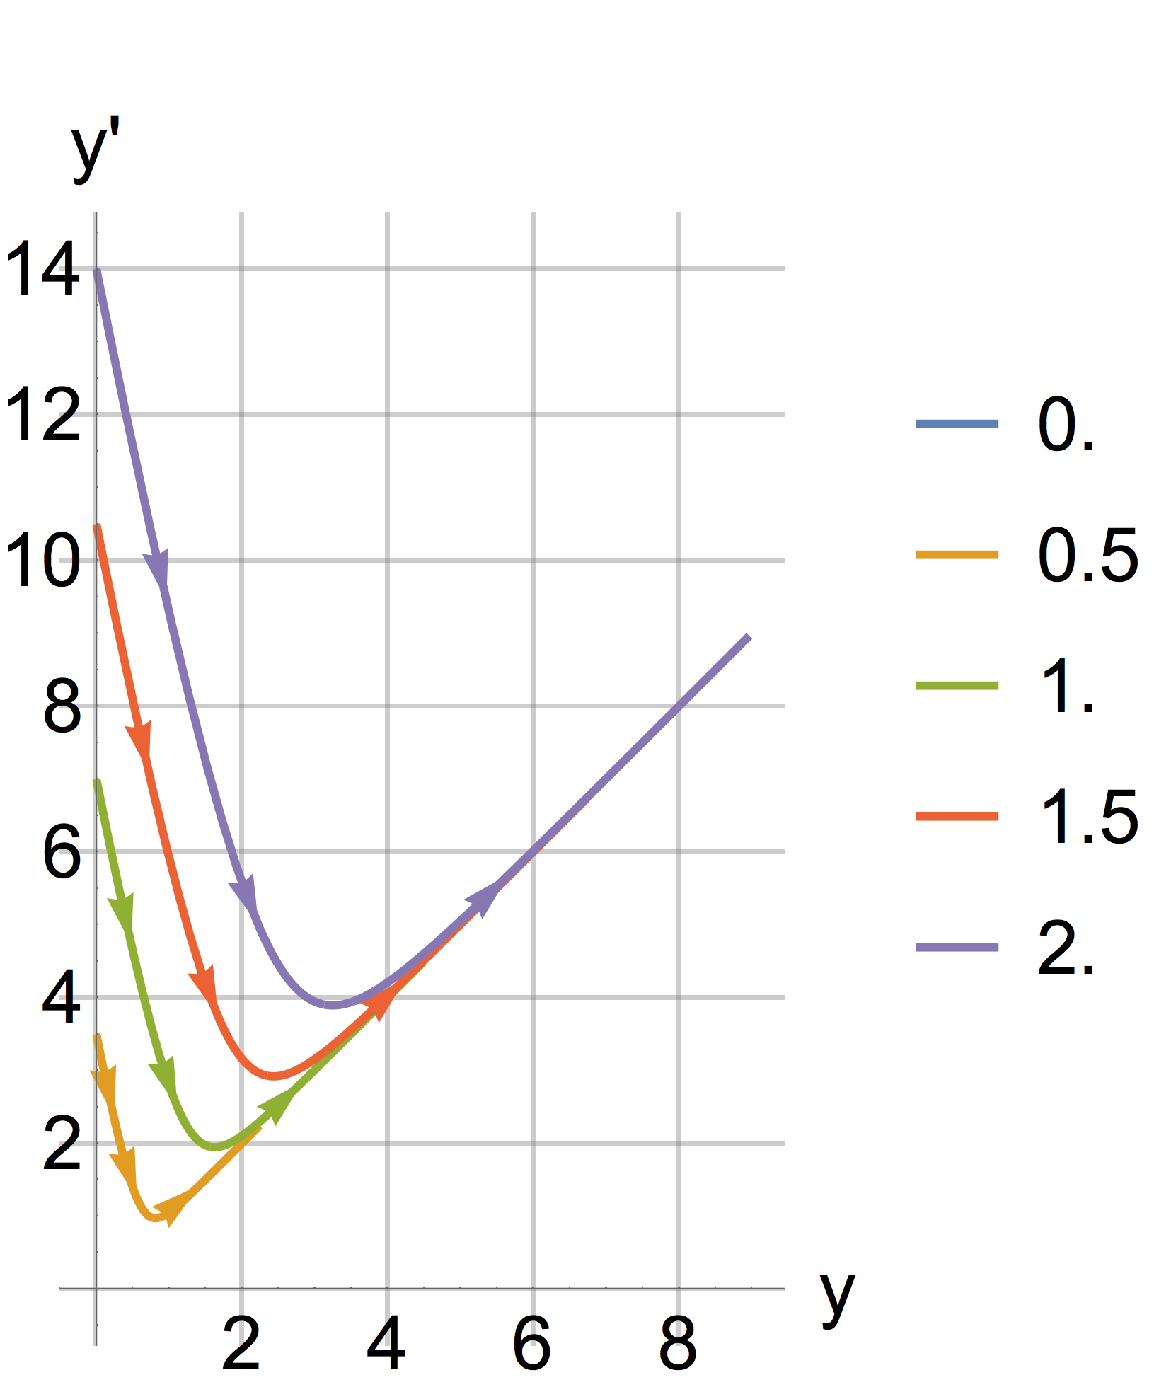
\includegraphics[scale=0.7]{phase_space_1.png}

You can note that as $t$ increases, the term $e^{-6t}$ goes to zero leaving the $e^t$ dominant, and since this features in both $y$ and $y'$, you get $y \propto y'$ for large $t$. % NT: Check this: As expected for this negatively-damped equation, both the velocity and position increase rapidly with time.

The examples we are considering here are relatively simple, however this can be used to identify complex and chaotic phenomena visually. For example, considering a pendulum gently swinging backwards and forwards, it is possible to trace out the phase-space as shown here:

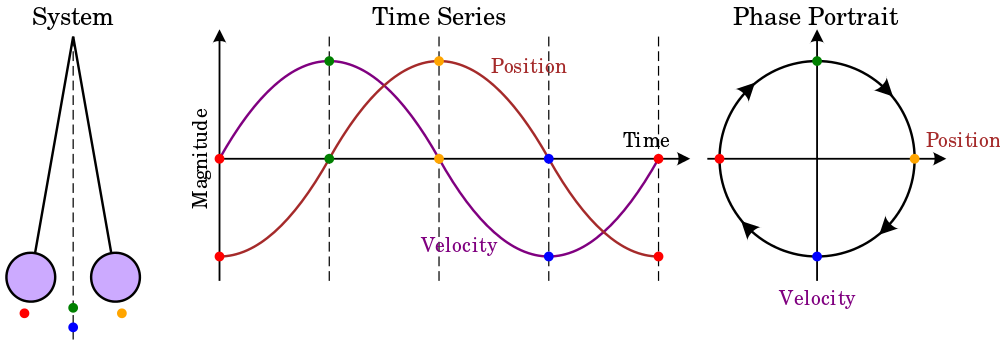
\includegraphics[scale=0.4]{pendulum_gentle.png}\\
\emph{\small{Source: \url{https://commons.wikimedia.org/wiki/File:Pendulum_phase_portrait_illustration.svg}, Wikipedia user Krishnavedala}}

If you increase the speed of the pendulum, at some critical point, instead of swinging back to the original position it will start whirring round and round. Expressed in terms of vertical angle and angular velocity, the graph becomes:

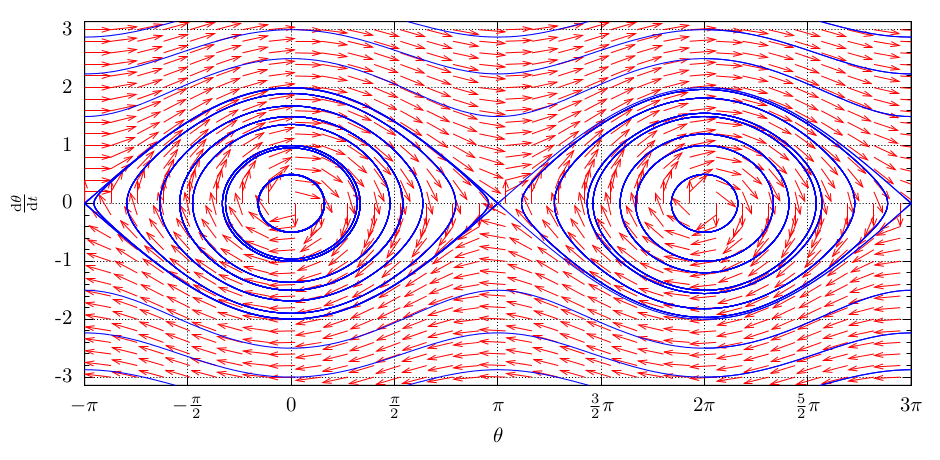
\includegraphics[scale=1]{pendulum_fullphase.png}\\
\emph{\small{Source: \url{https://commons.wikimedia.org/wiki/File:Pendulumphase.png}}}

At low velocities the pendulum swings back and forth (blue circles, angular velocity both positive and negative), but at high velocities, the angular velocity stays positive (or negative) and the pendulum whirs round and round in one direction (blue wavy lines). Note that position $\theta = \pi$ is when the rigid pendulum is pointing exactly upwards. So with no momentum it is stationary here, albeit unstable, because with a tiny velocity it will perform a full loop, slowing (but not stopping) as it reaches the top again.

\subsection*{Challenge}
1. The graphs below represent the solutions to the exercises 1-5 in challenge \ref{sec:systemsolving}.
Place the graphs below in the same order as exercises 1-5. Note that in order to maintain clarity, the graphs are not necessarily plotted over the same time interval $t$.

\begin{tabular}{cc}
    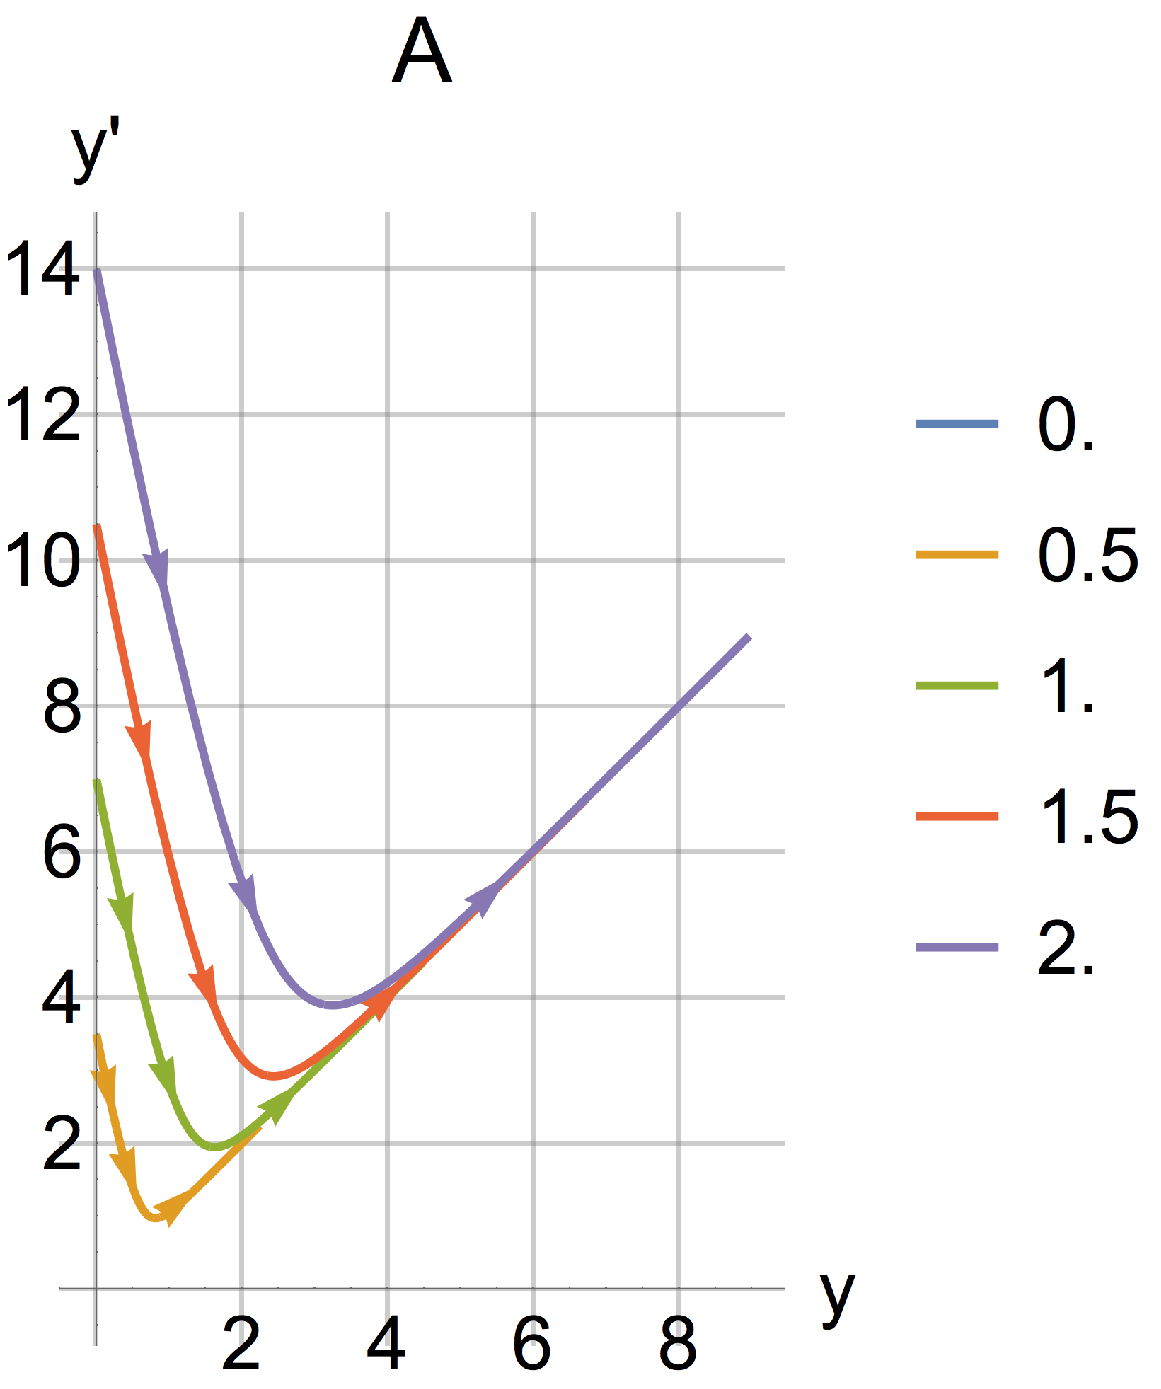
\includegraphics[scale=0.6]{phase_space_a.png} &
    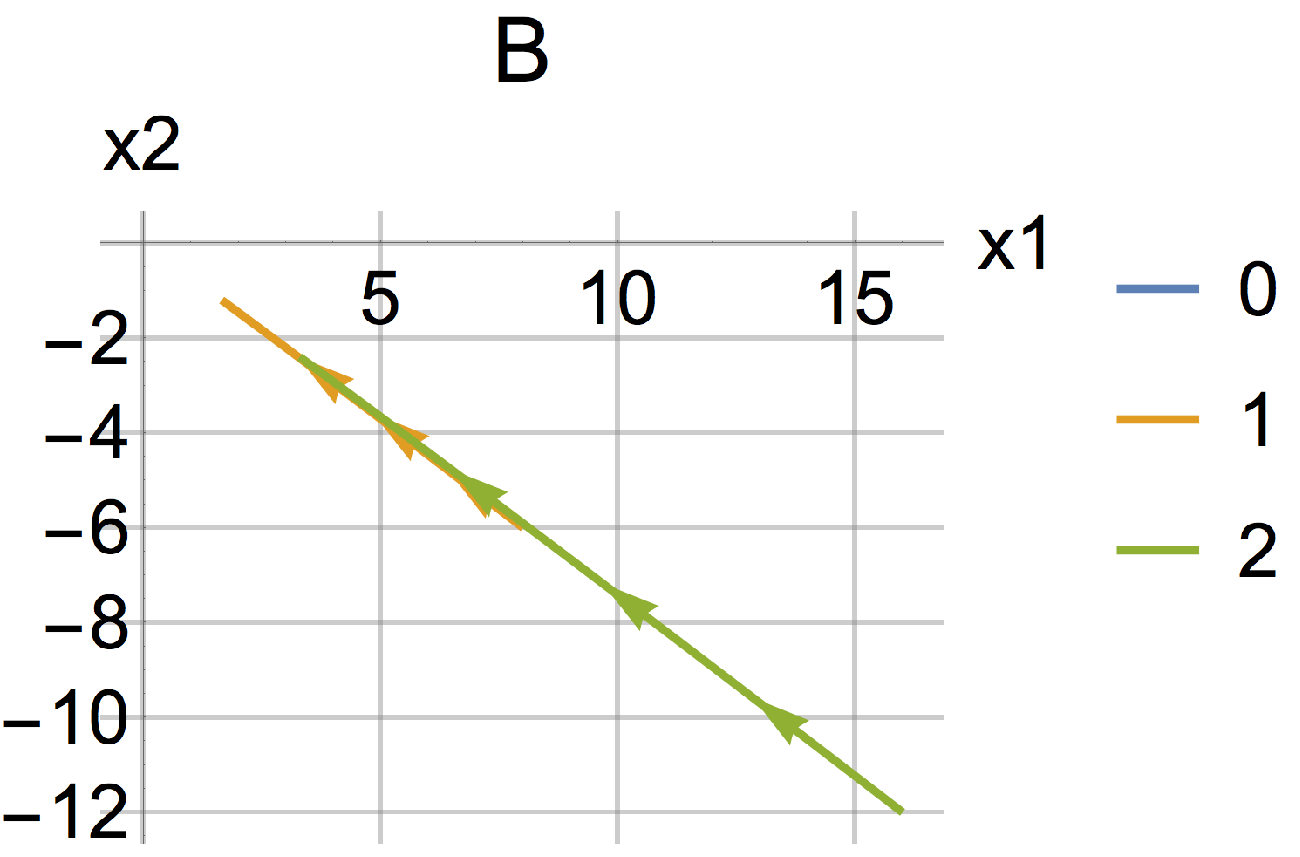
\includegraphics[scale=0.6]{phase_space_b.png} \\
    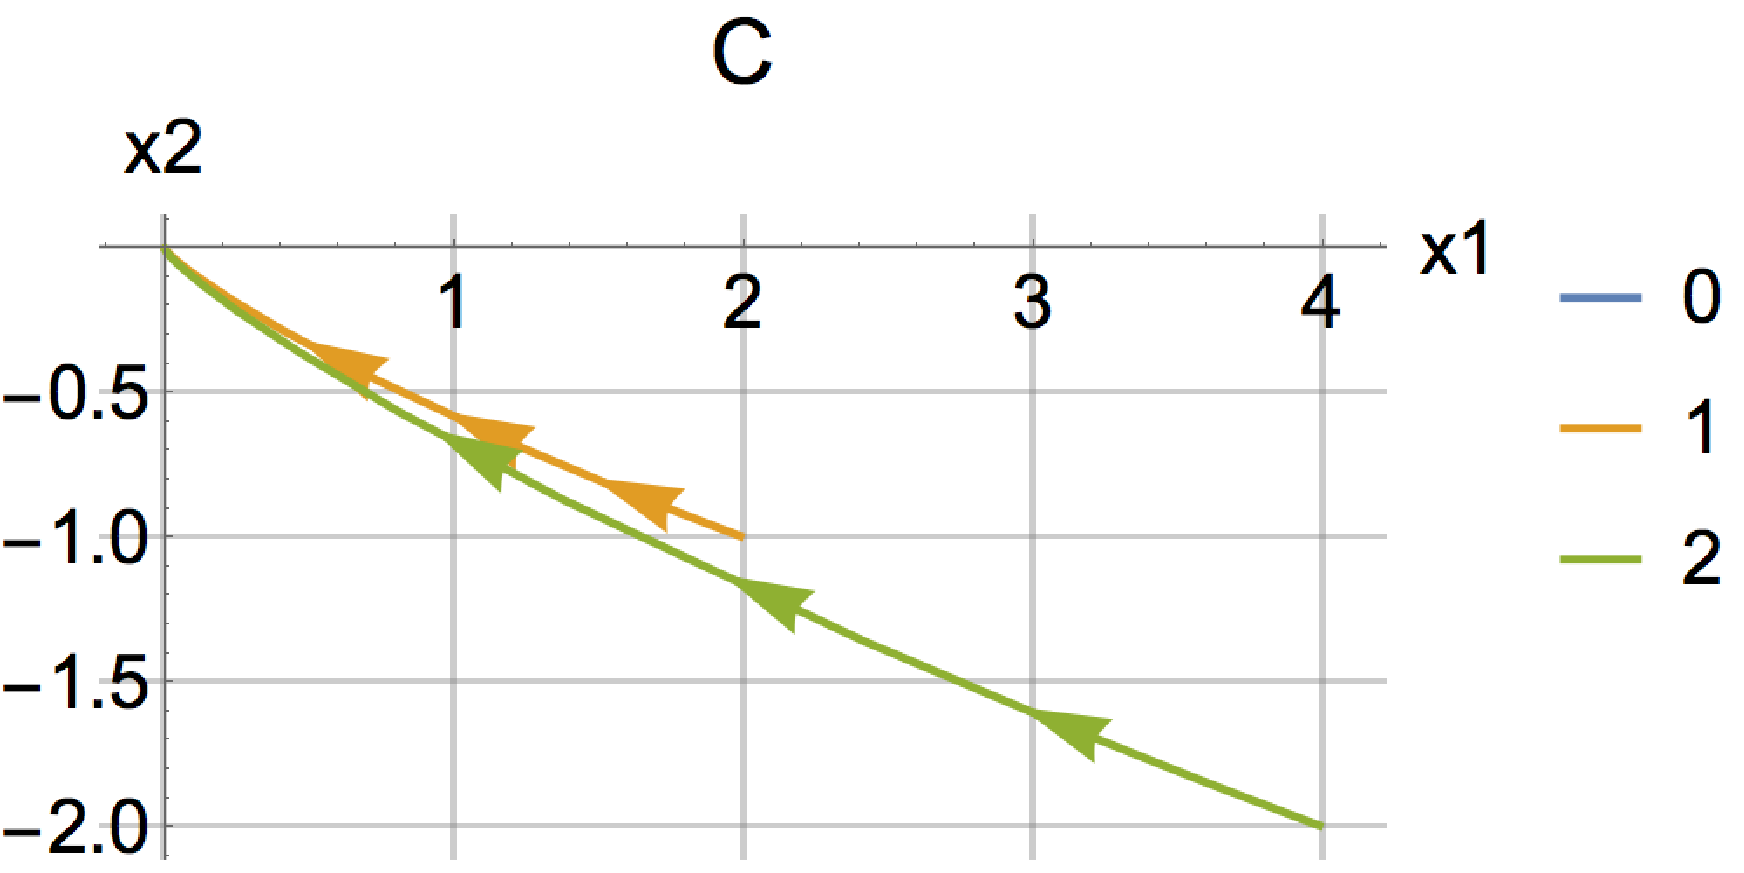
\includegraphics[scale=0.6]{phase_space_c.png} &
    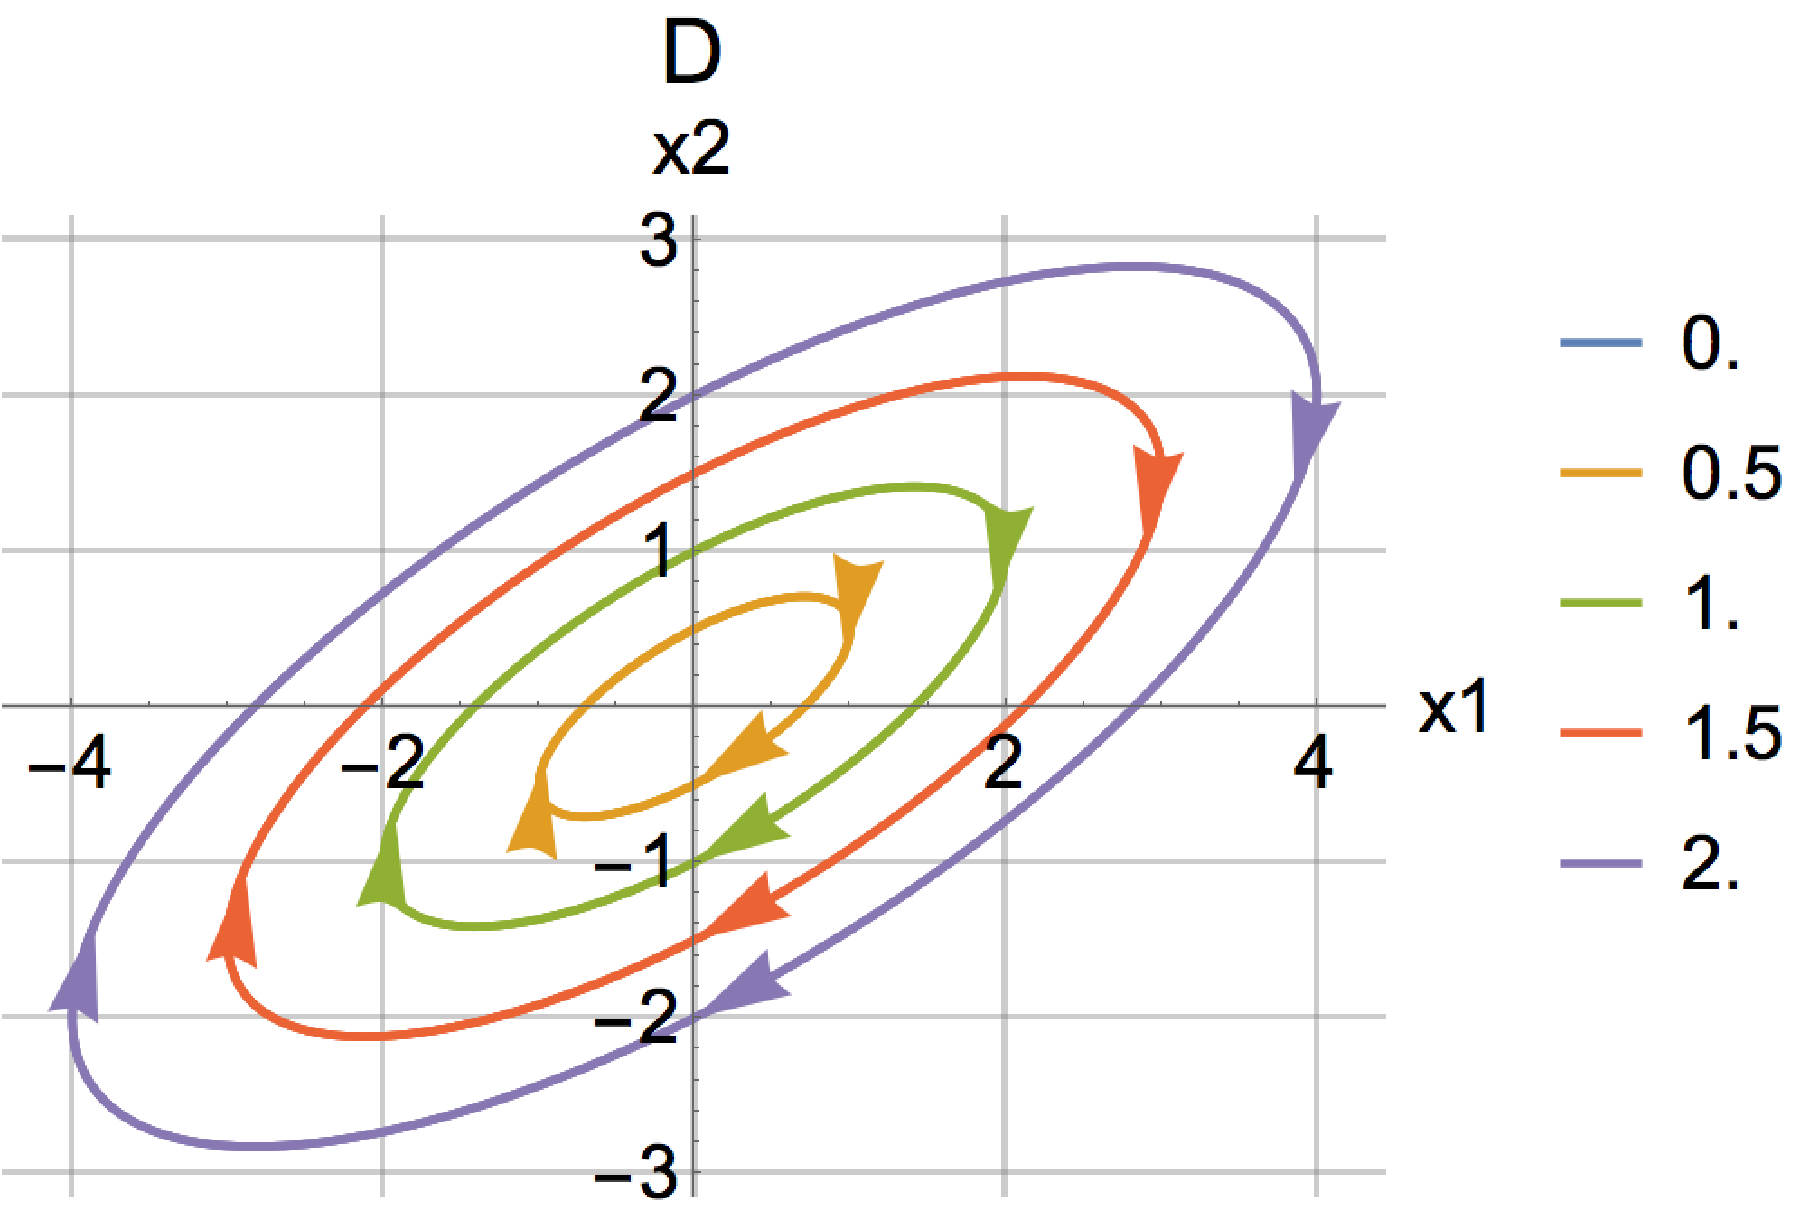
\includegraphics[scale=0.5]{phase_space_d.png} \\
    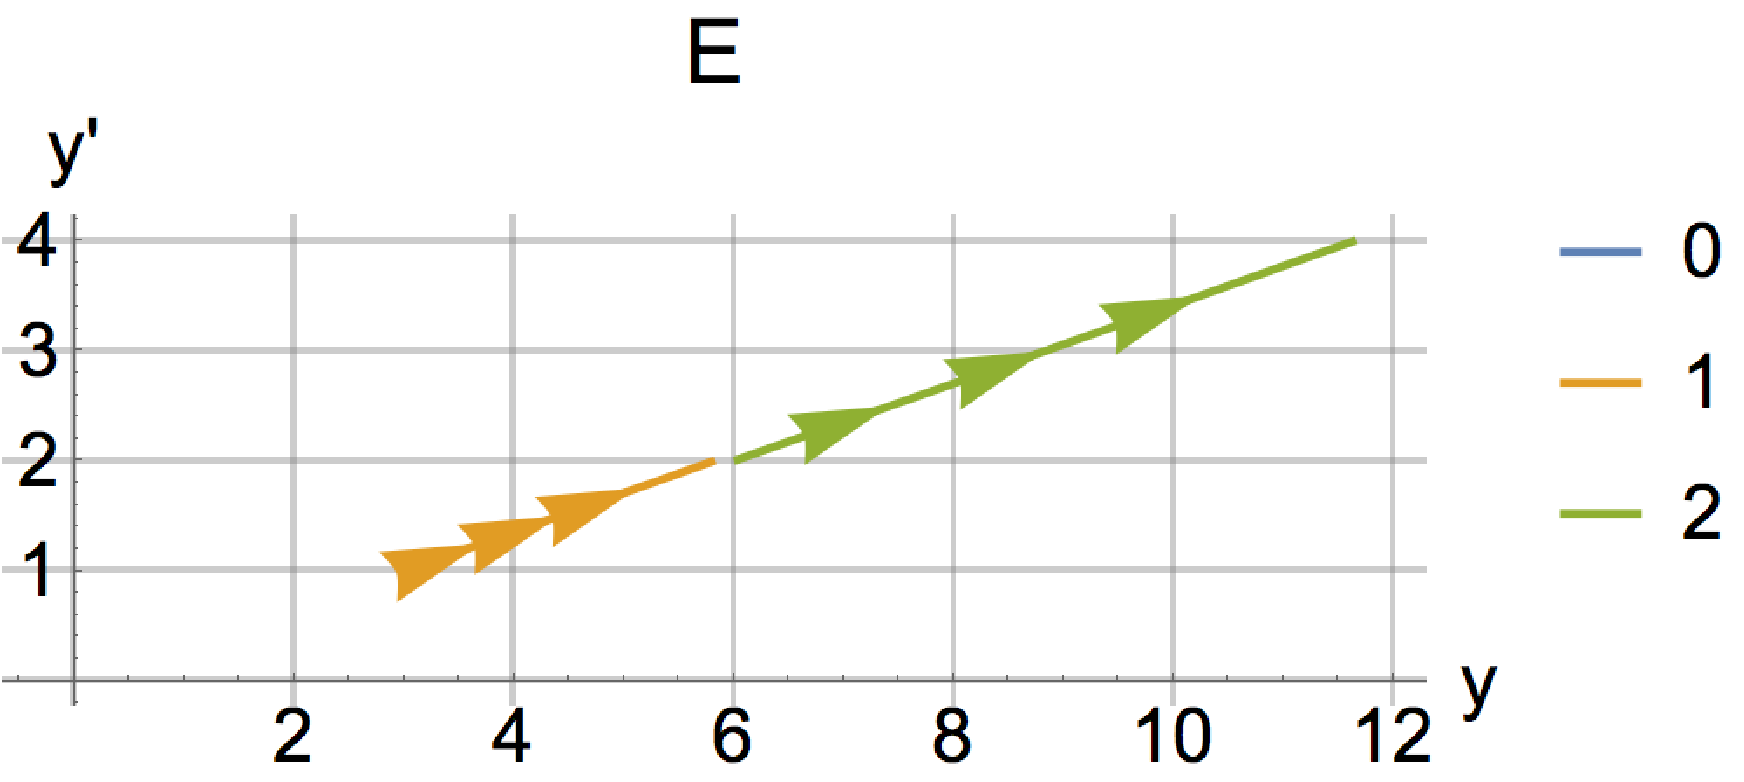
\includegraphics[scale=0.6]{phase_space_e.png} &
\end{tabular}
% NT: Add graphs that have the same starting position so students need to check the shape of the graph, as well as the t=0 position

\vspace{1cm}
2. Considering the graph shown earlier of angular momentum vs angle for a rigid pendulum, add the points of the following true statements:

\textbf{1 point} An initial angular velocity of 1 unit results in whirring circular motion irrespective of the starting angle.

\textbf{2 points} An initial angular velocity of -2.5 units results in whirring circular motion irrespective of the starting angle.

\textbf{4 points} An initial angle of $\pi/2$ combined with an angular velocity of 1 unit results in periodic swinging motion.

\textbf{8 points} An initial angle of $\pi/2$ combined with an angular velocity of 1 unit results in circular whirring motion.

\textbf{16 points} An initial angle of $0$ combined with an angular velocity of 0 units results in periodic swinging motion.

\textbf{32 points} An initial angle of $0$ combined with an angular velocity of 0 units results in a stationary system.

\textbf{64 points} An initial angle of $\pi$ combined with an angular velocity of 0 units results in a stationary system.

\textbf{128 points} An initial angle of $\pi/2$ combined with an angular velocity of 0 units results in a stationary system.

\textbf{256 points} An initial angular velocity of 3 units results in whirring circular motion in the same direction as an initial angular velocity of -3 units.

\textbf{512 points} An initial angular velocity of 3 units results in whirring circular motion in the opposite direction as an initial angular velocity of -3 units.

\subsection*{Solutions}

1. (eg, ``abcde'') \hash{jjj}{778bbb}


2. (enter number to 2 decimal places, as usual) \hash{kkk}{7febe0}


% NT: bifurcation? https://en.wikipedia.org/wiki/Hopf_bifurcation
% Other Pendulum resources of interest: http://math.stackexchange.com/questions/666806/nonlinear-pendulum and https://www.youtube.com/watch?v=6KSXLGHsrrs
